\vspace{-1.6em}
\section{Introduction}
\label{sec:intro}


In recent years, substantial progress has been achieved in the development of models for short-video representation learning. Numerous  \cite{zhu2024languagebind, Wang2024InternVideo2SV, Chen2023VASTAV, Xue2022CLIPViPAP, Luo2021CLIP4ClipAE, Lin2023VideoLLaVALU, Li2023LLaMAVIDAI, Xu2024PLLaVAP, Yang2023Vid2SeqLP} approaches have been introduced, demonstrating state-of-the-art performance across various tasks such as video classification, action recognition, text-video retrieval, video captioning, and video question answering. 

While models targeting short video clips (5–15 seconds long) are effective at capturing isolated moments, atomic actions, or specific events, they usually struggle to capture long-range temporal dependencies essential for understanding complex, extended narratives. For example, grasping the full emotional journey of characters in a drama or following the progression of a complex plot in a movie often requires viewing the entire film, not just a brief scene. 


Meanwhile, developing models that can effectively handle long video content (\eg, 20 minutes long) remains a significant challenge. 
First, most current methods process spatio-temporal tokens at the frame level, restricting the input video length they can handle.
Second, scaling these methods to accommodate longer sequences becomes computationally prohibitive, as training on extended videos demands significant GPU memory, along with increased training cost and time, limiting accessibility for many researchers and organizations.
Third, annotating long videos requires substantial effort, and defining unambiguous annotation guidelines is challenging, often leading to inconsistencies.

\begin{figure*}[t!]
    \centering
    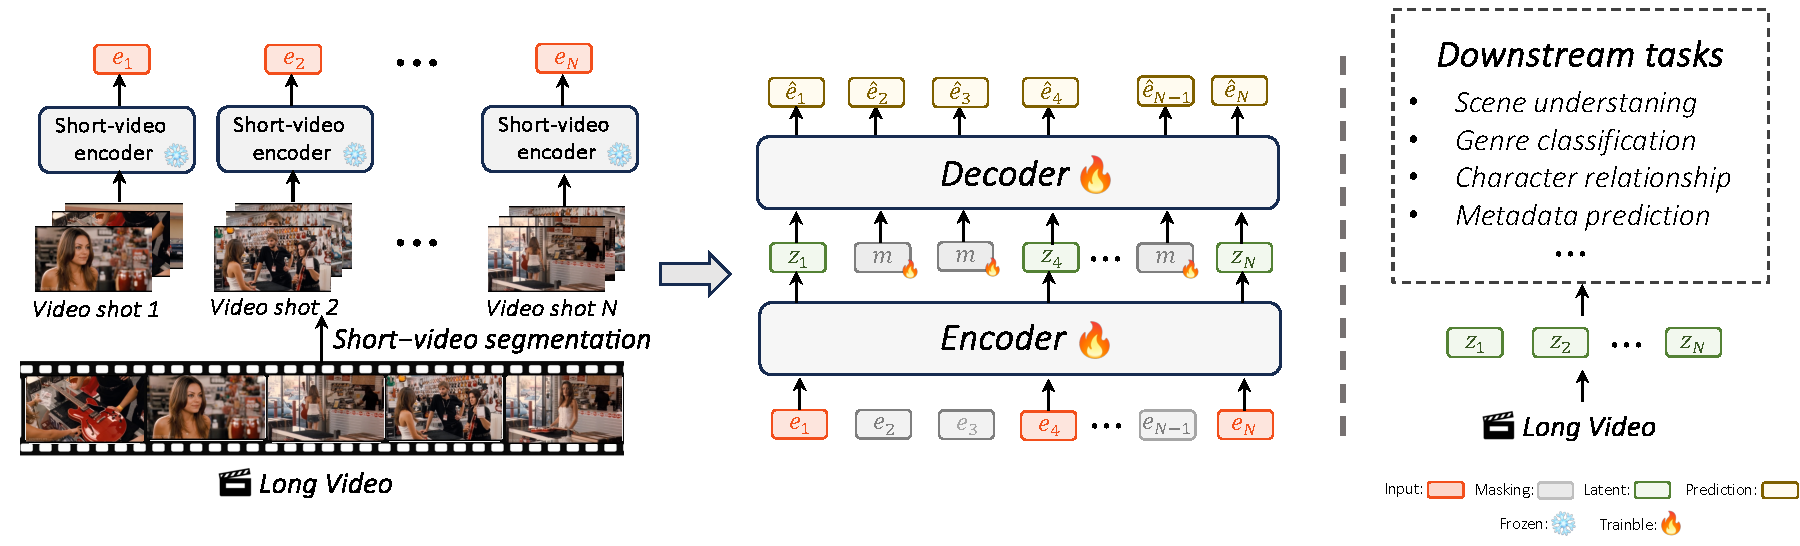
\includegraphics[width=.95\textwidth]{figures/arch_method.pdf}
    \caption{\textbf{Overview of the LV-MAE method.} LV-MAE first utilizes short-video representations extracted by advanced multimodal off-the-shelf encoders (\eg, LanguageBind~\cite{zhu2024languagebind}, InternVideo2~\cite{Wang2024InternVideo2SV}) to capture low-level knowledge of atomic actions and localized events. Next, we pre-train a masked embedding autoencoder to learn long-range dependencies across video segments in a self-supervised manner. After pre-training, the LV-MAE encoder is used to extract high-level representations for long-video downstream tasks.}
    \label{fig:arch}
\end{figure*}

Recently, approaches for handling long-video content have been proposed based on state-space models (SSMs) to address some of the above challenges. ViS4mer~\cite{islam2022long} utilizes a transformer encoder to extract patch-level features from each individual frame, followed by an efficient aggregation of these representations across all frames using the S4 decoder~\cite{gu2022efficiently}. VideoMamba~\cite{li2024videomamba}, a fully SSM-based video model, directly processes spatio-temporal patches from video frames using multiple bidirectional Mamba blocks~\cite{Zhu2024VisionME}. 
These architectures successfully bypass the quadratic complexity of the transformer's attention mechanism and are trained on sequences of up to 64 frames~\cite{islam2022long, li2024videomamba}. Yet, their computational demands rise significantly when applied to videos of extended duration.





In this paper, we tackle the challenges of learning representations for long video content by proposing a self-supervised approach to pre-train on videos ranging from minutes to hours.

Our method is not constrained by the number of frames and is highly efficient in terms of training cost.
Our key idea is to decouple the extraction of low-level representations, which can be effectively achieved using high-performing off-the-shelf short-video models, from the task of modeling long-range dependencies across short video segments. 


Specifically, we propose Long-Video MAE (LV-MAE), a transformer-based architecture that uses representations extracted from a sequence of short video segments by off-the-shelf models to learn high-level, long-video representations through self-supervised training.
Our approach begins by segmenting a long video into short clips (\eg, five seconds long) and utilizing a multimodal model (\eg, LanguageBind~\cite{zhu2024languagebind}, IntenVideo2~\cite{Wang2024InternVideo2SV}), pre-trained for video-text alignment, to extract low-level embeddings for each segment. We then train a masked-embedding autoencoder that operates on these low-level embedding tokens to learn a high-level representation of the entire video.
In particular, we adopt the asymmetric encoder-decoder design from~\cite{he2022masked} and demonstrate that reconstructing masked embeddings effectively captures general high-level semantic knowledge across extended video sequences.
Furthermore, we employ a padding strategy and leverage masked self-attention to accommodate videos of arbitrary length.
An overview of the LV-MAE method is provided in~\cref{fig:arch}.


To highlight the difference between our approach and existing methods, consider the tokens required to process a two-minute long video: while frame-level approaches like ViS4mer~\cite{islam2022long} and VideoMamba~\cite{li2024videomamba} require 11,760 tokens (60 frames $\times$ 14 $\times$ 14 patches for a standard 16 $\times$ 16 image grid), our approach processes only 24 tokens in total, with one token per five-second segment.
This significantly reduces the computational burden on the self-attention layer, which has quadratic complexity. 
Furthermore, our method unlocks the capacity to handle a significantly larger number of frames, potentially reaching thousands. Additionally, we bypass the challenge posed by the lack of annotated long-video datasets, as existing datasets contain only short samples of a few minutes. 

A key contribution of our work is enabling pre-training on substantially longer video samples through self-supervised learning. We pre-trained LV-MAE on a large and diverse dataset comprising long-length movies and TV series. Our LV-MAE approach is highly efficient to train, requiring only 2.5 days on a single NVIDIA A10 GPU and 20 hours on 8 NVIDIA A10 GPU.


LV-MAE effectively learns long-range dependencies that generalize well to various downstream tasks. By leveraging the representations learned through LV-MAE, we achieve state-of-the-art performance with simple attentive probing~\cite{yu2022coca} or even linear probing across three long-video benchmarks: LVU~\cite{wu2021towards}, COIN~\cite{tang2019coin}, and Breakfast~\cite{kuehne2014language}. Additionally, we provide interpretable visualizations that monitor the quality of the pre-trained encoder by utilizing the aligned text-video space of the short-video encoder. Specifically, for each reconstructed masked token, we perform retrieval against a large set of captions, resulting in high-quality matches demonstrating the ability to reconstruct the semantic meanings of the masked embeddings. 

Our contributions are summarized as follows: (1) We introduce LV-MAE, a method for learning long-range dependencies across short-video segments by pre-training masked-embedding autoencoders on very long video samples (\eg, 20+ minutes). 

Our method is highly efficient to train and enables the processing of much longer videos by alleviating the constraint on the number of frames.
To the best of our knowledge, this is the first approach to apply masked autoencoders on sequences of embedding vectors instead of image patches.
(2) Leveraging LV-MAE representations, we achieve state-of-the-art results with minimal fine-tuning, using techniques such as attentive or linear probing, on three long-video downstream tasks: LVU~\cite{wu2021towards}, COIN~\cite{tang2019coin}, and Breakfast~\cite{kuehne2014language}. (3) By exploiting the video-language shared space of the short-video encoder, we introduce an interpretable technique to visualize how semantic knowledge is reconstructed within the LV-MAE encoder.